\begin{figure}[H]
    \centering
    
    % 1. STŘEDOVÁ OBDÉLNÍKOVÁ METODA
    \begin{minipage}{0.32\textwidth}
        \centering
        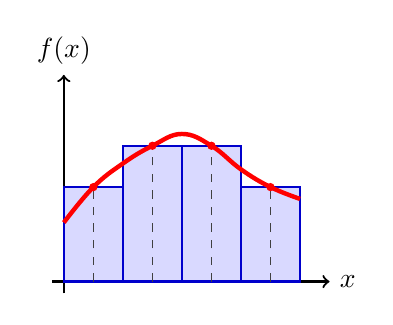
\begin{tikzpicture}[scale=0.75]
            % Osy
            \draw[->, thick] (-0.2, 0) -- (4.5, 0) node[right] {$x$};
            \draw[->, thick] (0, -0.2) -- (0, 3.5) node[above] {$f(x)$};
            
            % Obdélníky (výška určena středem intervalu)
            % Středy: 0.5 (y=1.6), 1.5 (y=2.3), 2.5 (y=2.3), 3.5 (y=1.6)
            \filldraw[fill=blue!15, draw=blue!80!black, thick] (0, 0) rectangle (1, 1.6);
            \filldraw[fill=blue!15, draw=blue!80!black, thick] (1, 0) rectangle (2, 2.3);
            \filldraw[fill=blue!15, draw=blue!80!black, thick] (2, 0) rectangle (3, 2.3);
            \filldraw[fill=blue!15, draw=blue!80!black, thick] (3, 0) rectangle (4, 1.6);
            
            % Vyznačení středů
            \foreach \x/\y in {0.5/1.6, 1.5/2.3, 2.5/2.3, 3.5/1.6} {
                \draw[dashed, darkgray] (\x, 0) -- (\x, \y);
                \fill[red] (\x, \y) circle (2pt);
            }
            
            % Samotná spojitá funkce
            \draw[ultra thick, red] plot [smooth, tension=0.7] coordinates { 
                (0,1) (0.5,1.6) (1,2) (1.5,2.3) (2,2.5) (2.5,2.3) (3,1.9) (3.5,1.6) (4,1.4) 
            };
        \end{tikzpicture}
        \caption*{Obdélníková (středová)}
    \end{minipage}\hfill
    %
    % 2. LICHOBĚŽNÍKOVÁ METODA
    \begin{minipage}{0.32\textwidth}
        \centering
        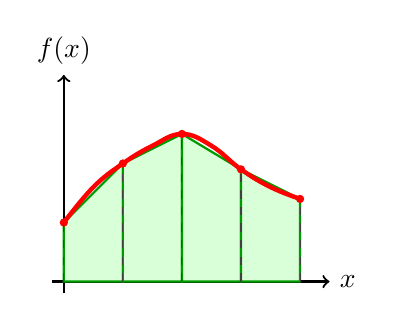
\begin{tikzpicture}[scale=0.75]
            % Osy
            \draw[->, thick] (-0.2, 0) -- (4.5, 0) node[right] {$x$};
            \draw[->, thick] (0, -0.2) -- (0, 3.5) node[above] {$f(x)$};
            
            % Lichoběžníky
            \filldraw[fill=green!15, draw=green!60!black, thick] (0,0) -- (0,1) -- (1,2) -- (1,0) -- cycle;
            \filldraw[fill=green!15, draw=green!60!black, thick] (1,0) -- (1,2) -- (2,2.5) -- (2,0) -- cycle;
            \filldraw[fill=green!15, draw=green!60!black, thick] (2,0) -- (2,2.5) -- (3,1.9) -- (3,0) -- cycle;
            \filldraw[fill=green!15, draw=green!60!black, thick] (3,0) -- (3,1.9) -- (4,1.4) -- (4,0) -- cycle;
            
            % Vyznačení uzlů
            \foreach \x/\y in {0/1, 1/2, 2/2.5, 3/1.9, 4/1.4} {
                \fill[red] (\x, \y) circle (2pt);
                \draw[dashed, darkgray] (\x, 0) -- (\x, \y);
            }
            
            % Samotná spojitá funkce
            \draw[ultra thick, red] plot [smooth, tension=0.7] coordinates { 
                (0,1) (0.5,1.6) (1,2) (1.5,2.3) (2,2.5) (2.5,2.3) (3,1.9) (3.5,1.6) (4,1.4) 
            };
        \end{tikzpicture}
        \caption*{Lichoběžníková}
    \end{minipage}\hfill
    %
    % 3. SIMPSONOVA METODA
    \begin{minipage}{0.32\textwidth}
        \centering
        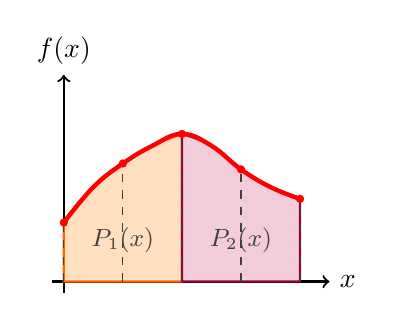
\begin{tikzpicture}[scale=0.75]
            % Osy
            \draw[->, thick] (-0.2, 0) -- (4.5, 0) node[right] {$x$};
            \draw[->, thick] (0, -0.2) -- (0, 3.5) node[above] {$f(x)$};
            
            % Simpson - první parabola (přes body 0, 1, 2)
            \fill[orange!25, draw=orange!80!red, thick] 
                (0,0) -- plot [smooth, tension=0.7] coordinates {(0,1) (0.5,1.6) (1,2) (1.5,2.3) (2,2.5)} -- (2,0) -- cycle;
            
            % Simpson - druhá parabola (přes body 2, 3, 4)
            \fill[purple!20, draw=purple!80!black, thick] 
                (2,0) -- plot [smooth, tension=0.7] coordinates {(2,2.5) (2.5,2.3) (3,1.9) (3.5,1.6) (4,1.4)} -- (4,0) -- cycle;
                
            % Svislé dělící čáry a uzly
            \foreach \x/\y in {0/1, 1/2, 2/2.5, 3/1.9, 4/1.4} {
                \draw[dashed, darkgray] (\x, 0) -- (\x, \y);
                \fill[red] (\x, \y) circle (2pt);
            }
            
            % Značky P1 a P2 pro paraboly
            \node[font=\small\bfseries, darkgray] at (1, 0.7) {$P_1(x)$};
            \node[font=\small\bfseries, darkgray] at (3, 0.7) {$P_2(x)$};
            
            % Samotná spojitá funkce
            \draw[ultra thick, red] plot [smooth, tension=0.7] coordinates { 
                (0,1) (0.5,1.6) (1,2) (1.5,2.3) (2,2.5) (2.5,2.3) (3,1.9) (3.5,1.6) (4,1.4) 
            };
        \end{tikzpicture}
        \caption*{Simpsonova (paraboly)}
    \end{minipage}
    
    \caption{Geometrická interpretace tří základních složených kvadraturních vzorců pro krok $h=1$. Červená křivka reprezentuje přesnou funkci $f(x)$. Obdélníková metoda využívá funkční hodnotu uprostřed podintervalu. Lichoběžníková metoda spojuje hranice úsečkou. Simpsonova metoda prokládá vždy trojicí bodů (dvěma podintervaly) parabolu ($P_1, P_2$).}
    \label{fig:integrace}
\end{figure}